\section{Theory}

\subsection{Coherent light}
Light is an electromagnetic wave characterized by oscillations of its electric field $\vec{E}(\vec{r},t)$ in space and time. 
The coherence of light describes how well different parts of this wave maintain a fixed phase relationship with each other.
In general, coherence quantifies the ability of light to produce stable interference patterns.
\noindent
There are two main types of coherence:
\begin{itemize}
    \item \textbf{Temporal coherence:} Measures how long (or over what path length) the phase relationship remains constant over time. It depends on the spectral width $\Delta\nu$ or wavelength spread $\Delta\lambda$ of the source. The corresponding quantities are the coherence time $\tau_c$ and coherence length $l_c = c\,\tau_c$.
    \item \textbf{Spatial coherence:} Describes how uniform the phase is across different points on a wavefront. High spatial coherence means that all parts can interfere with each other consistently.
\end{itemize} 
Coherent light therefore means that there exists a predictable and stable phase relationship between its electric field values at different positions and times. The coherence of light is a crucial factor for observing clear interference patterns when two light waves interfere with each other as it is necessary for this experiment. These patterns occur when waves with compatible phases interfere constructively or destructively. A laser beam, as used in this experiment, exhibits both high temporal and spatial coherence due to its narrow spectral width and well-defined wavefront.
\noindent
The quantitative measure for this property (or level of coherence) is given by the complex degree of coherence:
\begin{equation}
    \gamma_{1,2}(\vec{r}_1,t_1;\vec{r}_2,t_2)=
    \frac{\langle E(\vec{r}_1,t_1)\,E^*(\vec{r}_2,t_2) \rangle}
    {\sqrt{\langle |E(\vec{r}_1,t_1)|^2\rangle\,\langle |E(\vec{r}_2,t_2)|^2\rangle}}
    \label{eqn:degree}
\end{equation}
Here $E(\vec{r}_i,t_i)$ represents the complex amplitude of the electric field at position $\vec{r}_i$ and time $t_i$.
\noindent
Physically \autoref{eqn:degree} expresses how strongly correlated two field values are. If $\gamma_{1,2}=1$, their relative phase is perfectly stable what means full (perfect) coherence. If $\gamma_{1,2}=0$, their phases fluctuate randomly and they are completely incoherent. Intermediate values $0<|\gamma_{1,2}|<1$ indicate partial coherence.
\noindent
Thus, $\gamma_{1,2}$ quantifies both temporal and spatial correlations in the electromagnetic field and determines whether interference fringes can be observed clearly.

\subsection{Polarization of light}
\label{sec:k}
Light is an electromagnetic wave consisting of oscillating electric and magnetic fields that are perpendicular to each other and to the direction of propagation. 
The polarization of light describes the orientation and temporal behavior of the electric field vector $\vec{E}$ as the wave propagates.
Two typical types of polarization of light are linear and circular polarization. These two examples can be seen in \autoref{fig:polalin} and \autoref{fig:pola}. In both figures you can see the x-component and the y-component of a wave and how they add up to a resulting wave (red coloured) with a linear (\autoref{fig:polalin}) or with a circular polarization (\autoref{fig:pola}).  

\begin{figure}[h]
    \centering
    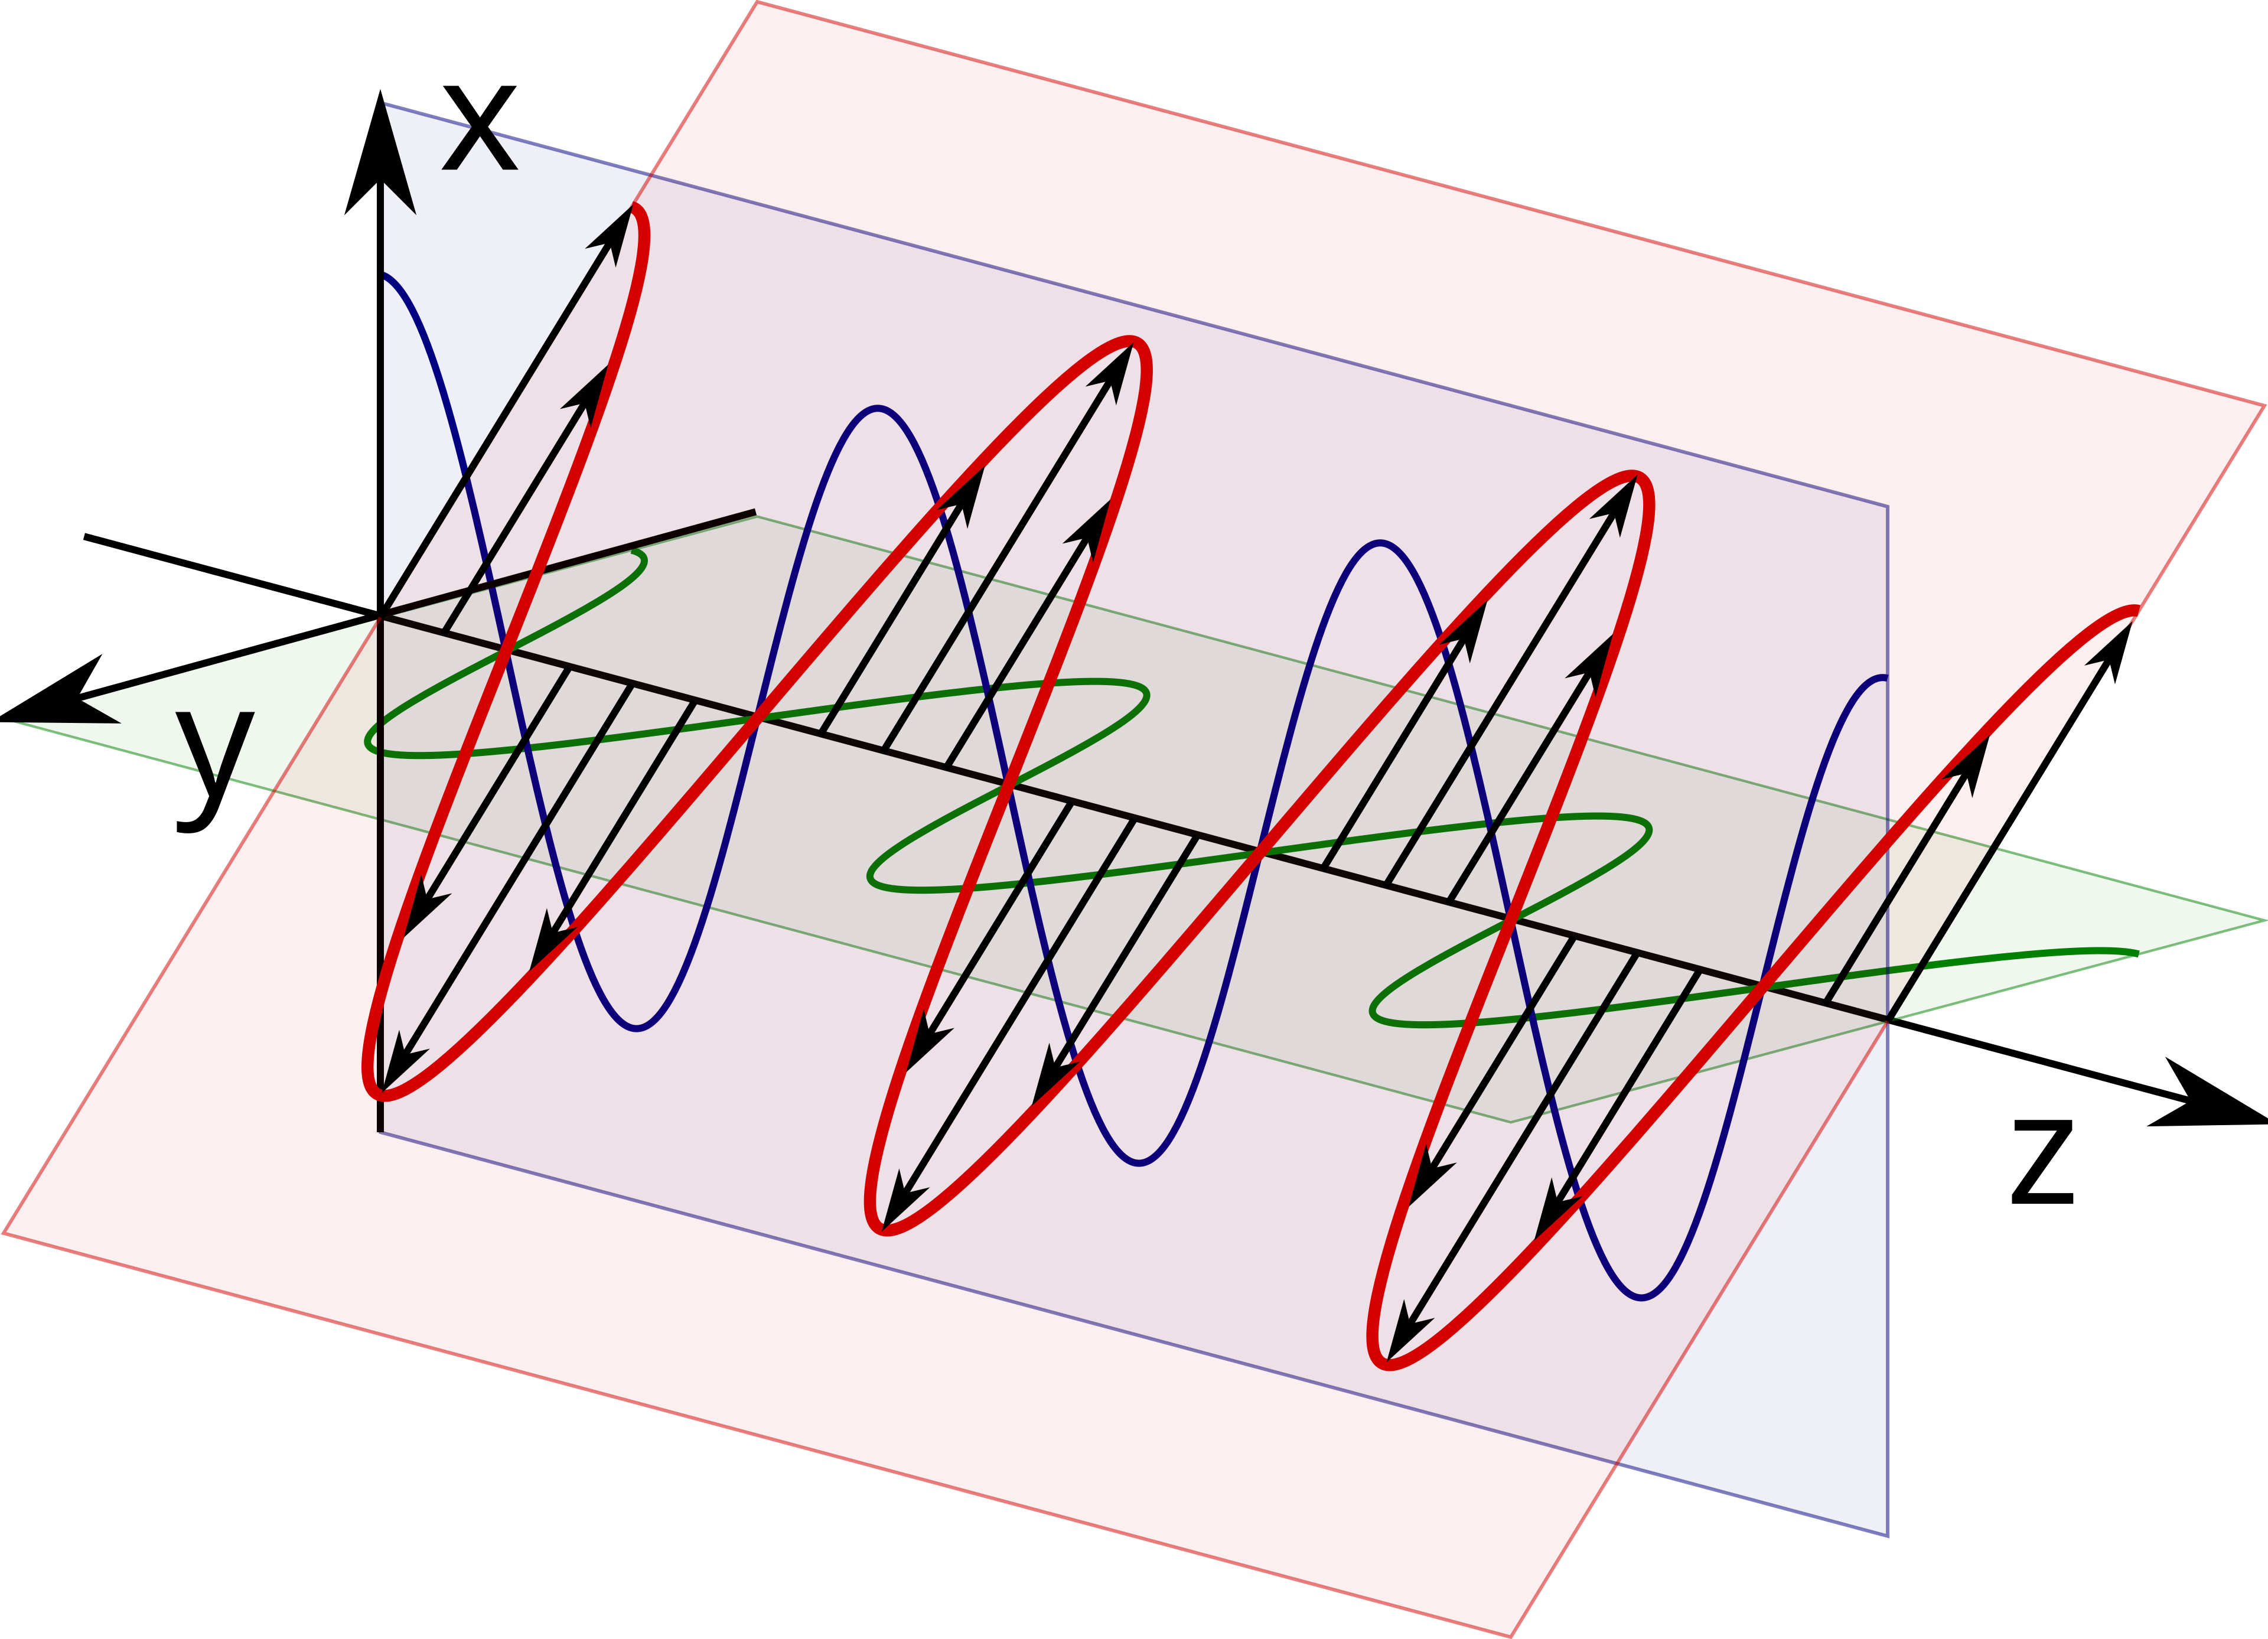
\includegraphics[width=0.7\textwidth]{plots/LinearPolarization.png}
    \caption{Linearly polarized wave \cite{pola}.}
    \label{fig:polalin}
\end {figure}
\noindent
In \autoref{fig:polalin} it can be seen that the the x and y components oscillate in phase and that the direction of oscillation for the resulting wave remains constant along the diagonal between the x and y axes.

\begin{figure}[h]
    \centering
    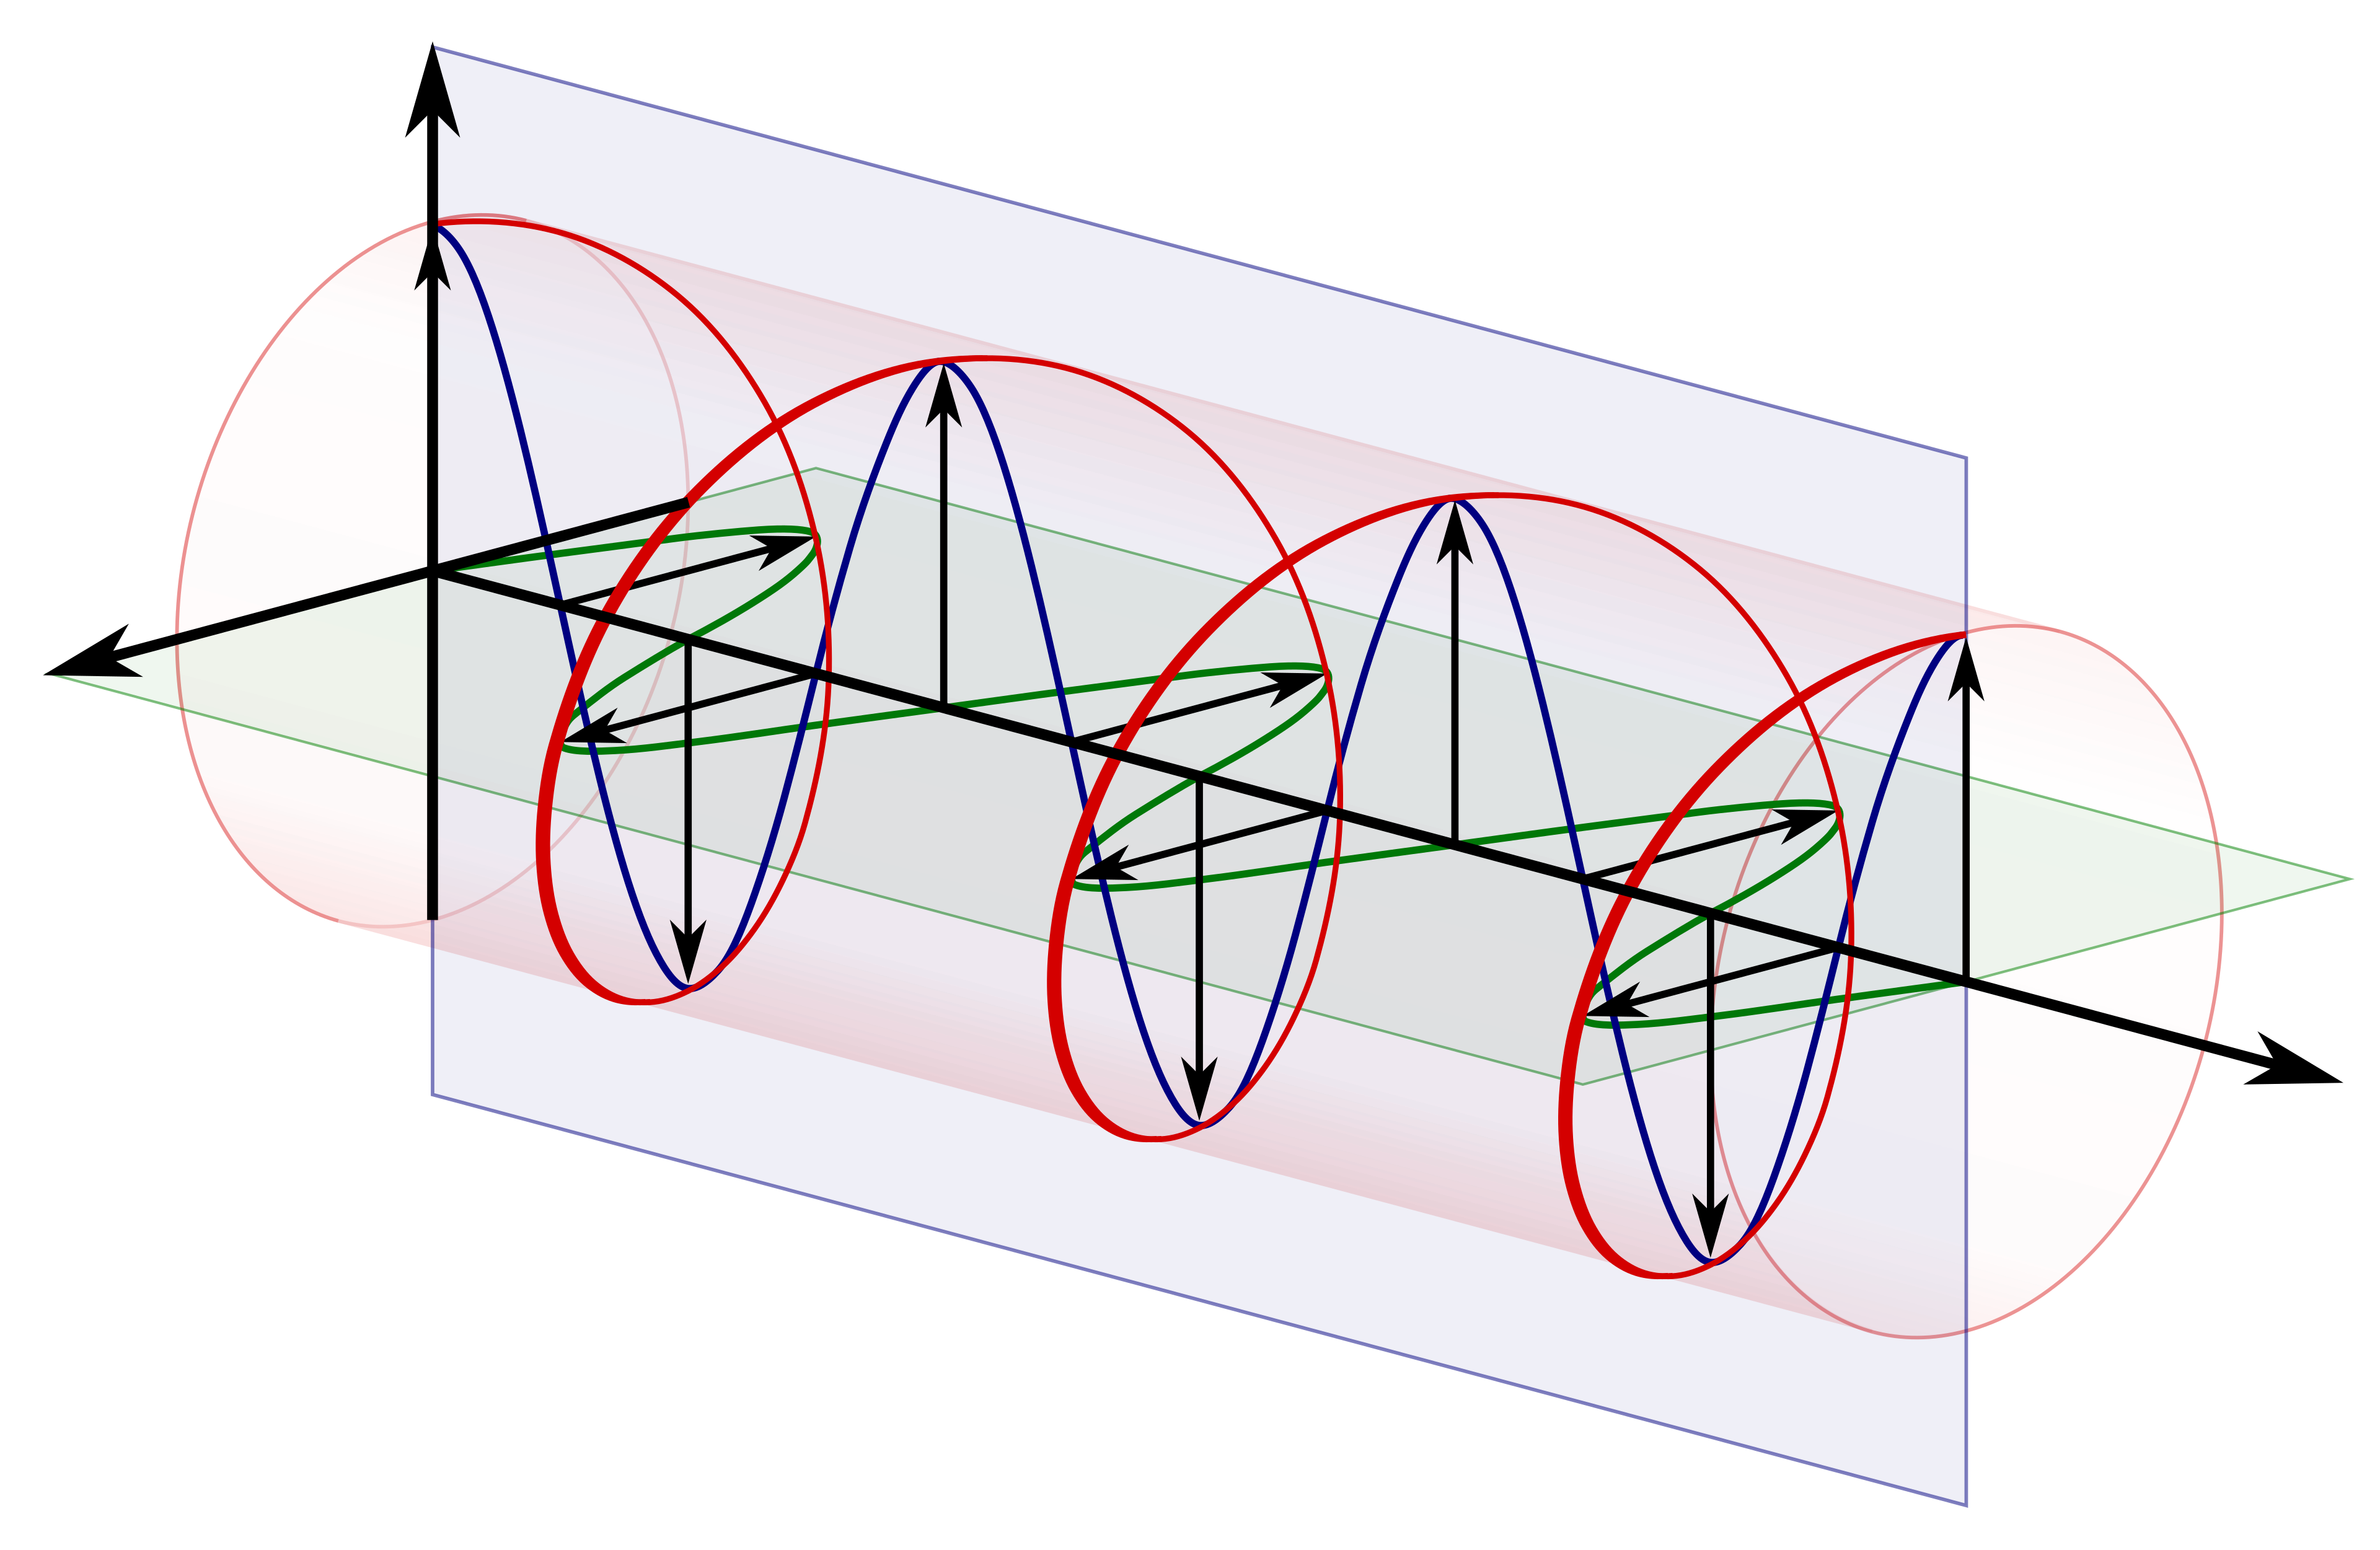
\includegraphics[width=0.7\textwidth]{plots/CircularPolarization.png}
    \caption{Circularly polarized wave \cite{pola}.}
    \label{fig:pola}
\end {figure}
\noindent
In \autoref{fig:pola} you can see that the the x and y components oscillate with a phase shift of 90 degrees and  that the direction of oscillation for the resulting wave rotates in this case.\newline
In general electromagnetic waves are oscillations in the electromagnetic field with different oscillation directions which determine their polarization. Unpolarized light typically consists of many different polarization directions. \newline
One possibility to get polarized light out of an unpolarized beam is letting it pass through a polarization filter, which only allows one specific polarization to pass through. Another way to get polarized light is to use a polarizing beam splitter cube (PBSC). Such a cube can reflect the s-polarized part of the light and transmit the p-polarized part of the beam. \newline
\noindent
The contrast $K$ of the interference pattern is defined as
\begin{equation}
  K = \frac{I_{\mathrm{max}}-I_{\mathrm{min}}}{I_{\mathrm{max}}+I_{\mathrm{min}}} \in [0,\, 1],
  \label{eqn:1}
\end{equation}
with 0 being the minimal contrast and 1 the maximum.
\newline
The total intensity $I$ resulting from two coherent waves can be written as
\begin{equation}
    I\propto \left\langle |E_1\cos(\omega t)+E_2\cos(\omega t +\delta)|^2 \right\rangle,
    \label{eqn:intensity}
\end{equation}
where $\omega$ is the angular frequency and $\delta$ is the phase difference between both waves.
\noindent
Expanding \autoref{eqn:intensity} gives

$$
I \propto E_1^2 + E_2^2 + 2E_1E_2\,\langle \cos(\omega t)\cos(\omega t+\delta)\rangle.
$$
\noindent
Using the trigonometric identity 
$\cos A\,\cos B = \tfrac12[\cos(A-B) + \cos(A+B)]$
and averaging over time (so terms oscillating with $2\omega t$ vanish), we obtain

$$
I \propto E_1^2 + E_2^2 + 2E_1E_2\,\tfrac12\,\cos(\delta),
$$
or equivalently,
\begin{equation}
I = C(E_1^2+E_2^2+ 2E_1E_2\,\cos({\delta})),
    \label{eqn:Iexpanded}
\end{equation}
where $C$ is a proportionality constant depending on experimental factors.
\noindent
From \autoref{eqn:Iexpanded}, it follows directly that:
\begin{itemize}
\item When $\delta = 0$, constructive interference occurs with maximum intensity:
  
$$
I_\text{max}\propto (E_1+E_2)^2 = E_1^2+E_2^2+ 2E_1E_2
$$

\item When $\delta = \pi$, destructive interference occurs with minimum intensity:
  
$$
I_\text{min}\propto (E_1-E_2)^2 = E_1^2+E_2^2 - 2E_1E_2
$$
\end{itemize}
\noindent
At this point we can assume that both interfering beams are linearly polarized under an angle $\phi$ relative to each other. In this case we can write the amplitudes of these waves as
\begin{align*}
    E_1&=E_0 \sin(\phi) \\
    E_2&=E_0 \cos(\phi).
\end{align*}
Then substituting these into our intensity expressions gives for the constructive and destructive cases:
\begin{equation}
    I_\text{max/min}\propto E_0^2 [\sin(\phi)^2 + \cos(\phi)^2 \pm 2\sin(\phi)\cos(\phi))].
\end{equation}
Because of $\sin(\phi)^2 + \cos(\phi)^2 =1$ this simplifies to

\begin{equation*}
    I_\text{max/min}\propto (1\pm 2\sin(\phi)\cos(\phi)).
\end{equation*}
These expressions can be inserted into our expression for the contrast $K$ (\autoref{eqn:1}) and by doing this we get for the numerator of $K$
\begin{equation*}
 I_\text{max} - I_\text{min} \propto [(1+2 \sin(\phi) \cos(\phi))-(1-2 \sin(\phi) \cos(\phi))] =4 \sin(\phi)\cos(\phi)
\end{equation*}
and for the denominator we get
\begin{equation*}
 I_\text{max} + I_\text{min} \propto [(1+2 \sin(\phi) \cos(\phi))+(1-2 \sin(\phi) \cos(\phi))] =2.
\end{equation*}
\noindent
Putting these expressions together in \autoref{eqn:1} we finally get for the contrast:
\begin{equation}
    K=2|\sin(\phi)\cos(\phi)|
    \label{eqn:k2}
\end{equation}

\subsection{Refractive indices}
\label{sec:ind}
The refractive index $n$ of a material quantifies how light propagates within that medium compared to in vacuum. 
It is defined as the ratio between the speed of light in vacuum $c$ and its phase velocity $v$ inside the material:
\begin{equation}
    n = \frac{c}{v}.
    \label{eqn:n_def}
\end{equation}
A larger refractive index means that light travels slower through the medium, which corresponds to stronger refraction when entering or leaving it.

\medskip
\noindent
When two coherent light waves pass through media with different refractive indices, they acquire a relative phase difference $\Delta\Phi$. 
This phase difference leads to an interference pattern consisting of intensity maxima and minima.
The number of these fringes $M$ is directly related to $\Delta\Phi$ by
\begin{equation}
    M = \frac{\Delta\Phi}{2\pi},
    \label{eqn:m}
\end{equation}
where one full $2\pi$ phase change corresponds to one complete fringe shift.
\noindent
For a plane-parallel glass plate of thickness $D$, tilted by a small angle $\theta$, the optical path difference between two interfering beams can be approximated as

$$
\Delta s(\theta) = D\,\frac{n-1}{2n}\,\theta^2,
$$
which yields a corresponding phase difference of
\begin{equation}
    \Delta\Phi(\theta) = 2\pi\,\frac{\Delta s(\theta)}{\lambda_\text{vac}} 
                      = 2\pi\,\frac{D}{\lambda_\text{vac}}\frac{n-1}{2n}\,\theta^2.
    \label{eqn:delta1}
\end{equation}
Because in this experiment the glass plates are symmetrically tilted by $\theta_0=\pm\SI{10}{\degree}$, 
the general expression for the phase shift from \autoref{eqn:delta1} can be simplified by replacing $\theta^2$, resulting in
\begin{equation}
    \Delta\Phi(\theta) = 2\pi\frac{D}{\lambda_\text{vac}}\frac{n-1}{n}\cdot 2\theta_0\theta.
\label{eqn:delta2}
\end{equation}
Then combining \autoref{eqn:m} and \autoref{eqn:delta2} gives an expression for the total number of observed interference fringes:
\begin{equation}
    M = 2\,\frac{D}{\lambda_\text{vac}}\frac{n-1}{n}\,\theta_0\,{\theta}
    \label{eqn:M_an}
\end{equation}
%Here, $\theta_0$ represents the tilt angle between the glass plates and changing $\theta$ modifies the optical path difference what shifts the interference fringes.
\noindent
Solving \autoref{eqn:M_an} for $n$ yields
\begin{equation}
    n =
        \frac{
            2 D\, {\theta_0}\, {\theta}}
             {2 D\, {\theta_0}\, {\theta} - {\lambda_{\mathrm vac}} M}.
       \label{eqn:n_glass}
\end{equation}
For gases the phase difference can be calculated by
\begin{equation*}
    \Delta\Phi=2\pi\frac{L}{\lambda_\text{vac}}(n-1).
\end{equation*}
Here $L$ is the length of the used gas chamber. Another way for the calculation of the refractive index of a gas depending on its pressure $p$ and temperature $T$ is the Lorentz-Lorenz law:
\begin{equation}
    \frac{n^2-1}{n^2+1}=\frac{Ap}{RT}
    \label{eqn:lll}
\end{equation}
Here $R$ represents the universal gas constant and $A$ represents the molar refractivity of the gas.